\def\year{2017}\relax
%File: formatting-instruction.tex
\documentclass[letterpaper]{article} %DO NOT CHANGE THIS
\usepackage{aaai17}  %Required
\usepackage{times}  %Required
\usepackage{helvet}  %Required
\usepackage{courier}  %Required
\usepackage{url}  %Required
\usepackage{graphicx}  %Required
\usepackage[ruled,vlined]{algorithm2e}
\frenchspacing  %Required
\setlength{\pdfpagewidth}{8.5in}  %Required
\setlength{\pdfpageheight}{11in}  %Required
%PDF Info Is Required:
  \pdfinfo{
/Title (Supervised Reinforcement Learning with Partial States: a Teaching Method for Action Selection for HRI)
/Author (Emmanuel Senft)}
\setcounter{secnumdepth}{0}  
 \begin{document}
% The file aaai.sty is the style file for AAAI Press 
% proceedings, working notes, and technical reports.
%
\title{Supervised Reinforcement Learning with Partial States: \\
 a Teaching Method for Action Selection for HRI}

\author{Emmanuel Senft \and S\'{e}verin Lemaignan\\
Centre for Robotics and Neural Systems \\
Plymouth University \\
United Kingdom\\
\And Paul Baxter\\
L-CAS\\
University of Lincoln\\
United Kingdom\\
 \And Tony Belpaeme\\
 CNRS\\ Plymouth University (UK) \\ iMinds \\ Ghent University (Be)}

\maketitle
\begin{abstract}
Robots are expected to be pervasive in human society in the future

not possible to hardcode everything by hand

requirement for learning

hard to learn for HRI
\begin{itemize}
	\item real time
	\item cost of exploration (real humans)
	\item no clear reward policy and cannot request a human to reward everything
	\item need to make the most out of each sample
\end{itemize}

Partial state RL - accelerate learning


\end{abstract}
%===============================================================================

\section{Introduction}

Robot interacting with humans, bla bla bla

State used for action selection can be from different sensors, continuous, discrete, representing a value or a state

\cite{kober2013reinforcement}
%===============================================================================

\section{Background}
\subsection{Reinforcement Learning}
\subsection{Human enhanced Reinforcement Learning}
One of the main challenge when applying RL to robotics is poor perfermance in
 the early stages of the learning as the agent has to explore the environment to
 gather initial knowledge. This challenge is especially
important for robotics as trials often have to happen in the real world (as
simulator close enough to the real world as not available) and as such can
present risks for the robot or for the persons interacting with it. 

%===============================================================================

\section{Proposition}
\subsection{Supervised Progressively Autonomous Robot Competencies}

As a way to enable a human supervisor to teach a robot an action policy while
interacting with its environment, we proposed the Supervised Progressively
Autonomous Robot Competencies (SPARC) in \cite{senft2015sparc}. SPARC is independent
of the learning algorithm used, but define an interaction dynamic between an
agent learning an action policy while interacting in an environment and a
supervisor teaching this agent an action policy. The main goal of SPARC is
enabling a robot to learn from a supervisor while ensuring that every action
executed by the robot has approval of the supervisor but without requiring this
supervisor to manually enforce every single action.

The main concept in SPARC is giving the supervisor the control over the agent
action and combine this with online learning on the agent side. This control is
achieved using a suggestion/correction mechanism whereas the agent is presenting
to the supervisor the action about to be executed and the supervisor can cancel
this action before its execution or not doing anything, letting the action being
executed after a delay. Additionally, the supervisor can select actions to be
executed by the agent. The actions selected or canceled by the supervisor can be
used as input with the current state by a learning algorithm to progressively
improve the future suggestions.

Giving power to an expert to correct the actions of the agent before the
execution can ensure that even in the early phases of the learning the agent can
have an appropriate action policy for the current environment as shown in Figure~\ref{fig:comparison}.

\begin{figure}
    \centering
    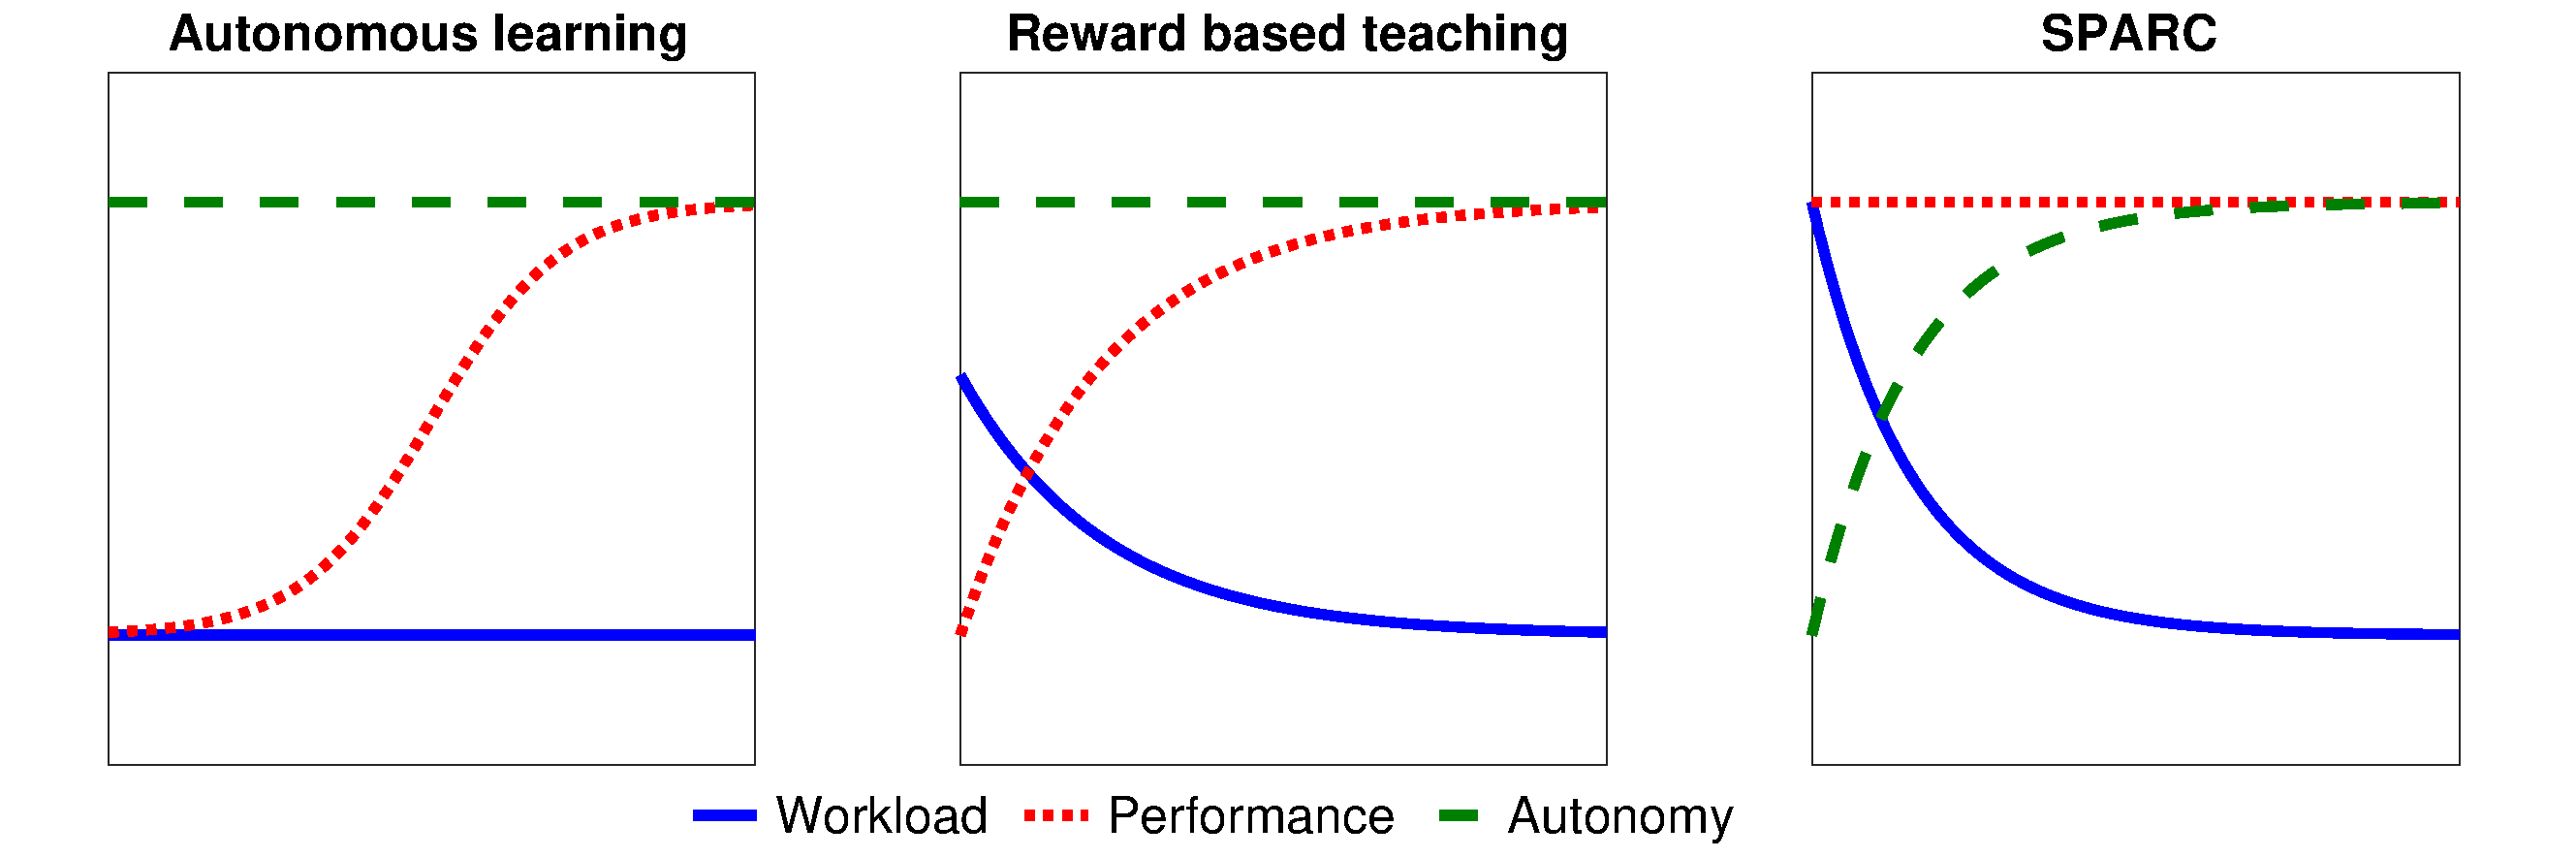
\includegraphics[width=0.9\linewidth]{./fig/motivation.pdf}
    \caption{Idealised expectation for performance, autonomy and workload for a
    Wizard of Oz, a autonomous learner and SPARC.}
    \label{fig:comparison}
\end{figure}

SPARC has been design with the idea of teaching a robot to interact with humans,
it is specially usefull when the pace of action selection is low (less than
1Hz), when the agent has to learn with a limited number of datapoints and when
undesired actions executed by an agent can have a high cost. 

In \cite{senft2017supervised}, we presented a way to combine SPARC and RL, by
assigning a positive reward to every action executed by the robot as it would
have been passively or actvely validated by the supervisor. However this method
was not making use of any type of generalisation, it was directly mapping a
single state action pair to a reward. 

\subsection{Partial-State Supervised Reinforcement Learning}

REFORMULATE: start with size of the world
To be usable in complex environments, a
learning algorithm requires generalisation as exactly identical spaces might
never been observed twice.

A classical approach to generalise in RL is to use a first layer of neural
network or to use deep reinforcement learning which relies on deep neural
networks to learn a mapping state-action-Qvalue for example. (ADDREF)
These approaches, neural network based, relies on having a large number of
datapoints to converge toward a good function approximator. However, as
discussed previously, in many application, these amounts of data are not
possible to be obtained and a robot might need to adapt to different persons and
be retrained quickly.

With that idea in mind, we propose to make a better use of human inputs, and ask
 the supervisor to identify which features of the environment are linked to the
 current selected action. That was, instead of having an state-action pair, we
 can have a partial-state action pair, with this partial-state being a subset of
 the state domain.

%===============================================================================
\section{Methodology}

\subsection{Supervisation}
Similarly to a SPARC setup, the supervisor is presented with action about to be
executed by the robot and can either cancel it or let it be executed and the 
supervisor has the possibility to select actions for the robot to execute.

In addition to these actions, the supervisor can use the GUI to select features
of the environment that can send to the algorithm to reduce the state associated
to this action to a partial-state. Similarly, the algorithm can indicate which
parts of the states have been used for the selection to the supervisor who can
correct them while the action is being executed.

Example?

\subsection{Learning algorithm}

In a first approach, the presence of an expert supervisor who can evaluate the
expected future impacts of an action removes the problem of credit assignment
for delayed rewards and allows us to consider only a myopic approach. (can cite
kobers I think.)

For this paper, we will reuse the formalism of rewardless Markov Decision 
Process to identify the different elements of our system. The agent has action
to a set of actions A, a state S (represented as a vector of n dimensions of
values $\in [0;1]$). With each dimension of S representing features in the
environment.

At the state $s_{t}$ the agent receives the action $a_{i}$ with the partial
state $s'$ defined in a subspace $S' \subseteq S$ (defined by selecting only a
number $n' \leq n$ of the dimensions of S). For example, a state s could be
defined in 4 dimensions such as $s=[1,0.2,0,0.5]$, and s' in two dimensions with
$s'=[-,0.2,0,-]$ with symbol '-' reprensenting the dimensions removed.

We store in memory the partial-state action pair $s'-a_{i}$, with the reward 1
as the action has been selected by the supervisor. Similarly, if an action has
been canceled by the supervisor, the partial-state action will be assigned to a
reward $-1$.

After interacting with the system under the supervisors control, the actions
will have associated to each action $a \in A$, a collection $C_{a}$ of pairs
partial-state-reward. When facing a new state $s$ where an action has to be
selected, the agent can select an action following Algorithm \ref{algo}.

\begin{algorithm}
    \DontPrintSemicolon
    \SetKwInOut{Input}{inputs}\SetKwInOut{Output}{output}
    \Input{Current state s, action-partial state rewards tuples}
    \Output{selected action $\pi(s)$}
    \ForEach{a $\in $ A}{
        \ForEach{ s'-r $\in C_{a}$}{
            compute similarity
            $\Delta(s',s)=1-\frac{\sum_{j}^{n'}(s'(j)-s(j))^{2}}{n'}$
        }
        $\Delta(a)=max(\Delta)$

        $r(a)=R(argmax_{s'} \Delta(s'))$
    }
    $\pi(s) = argmax_{a}\Delta(a) \cdot r(a)$

    \caption{Algorithm for selecting an action based on previous
    partial-state action rewards tuples and current state}
    \label{algo}
\end{algorithm}

When proposing an action following Algorithm~\ref{algo}, the agent can also use
the dimensions of the similar state s' to indicate the supervisor which parts of
the states have been used for the action selection.

%===============================================================================
\section{Results}

\section{Future work}

This method still has to be tested in a real Human-Robot Interaction, and this
evaluation is currently being implemented and will be tested in a near future.

Other way of extending the current work would be to combine it with the
possibility of letting the agent continue to explore in the absence of a
supervisor around a learnt action policy to keep improving its behaviour. This
could be done by allowing the supervisor to provide rewards during the learning
phase, rewards which could also be assigned to partial states. The system could
also learn to predict these rewards in an approach similar to TAMER 
\cite{knox2009interactively}. But in the case of an absence of supervisor, the assumption that only a
myopic action selection is sufficient would not hold anymore and the problem of
delayed rewards would have to be tackled. It could be for example possible to
adapt well known algorithms such as QLearning to handle partial states rather
the full states.

%===============================================================================
\section{Conclusion}
\label{sec:conclusion}
%==============================================================================
\section{Acknowledgments}
This work was supported by the EU FP7 DREAM project (grant no.  611391) and EU
H2020 Marie Sklodowska-Curie Actions project DoRoThy (grant 657227).  

\bibliographystyle{aaai} \bibliography{biblio}
\end{document}
